\subsection{Objektorientierte Programmierung}
In der Objektorientierten Programmierung mit Unity dreht sich alles um GameObjects. Jedes Objekt in der Szene, egal ob sichtbar oder nicht ist ein GameObject. Diese GameObjects können verschiedene Komponenten haben, welche Eigenschaften definieren, also Daten speichern. Diese Komponenten sind jedoch nicht zu verwechseln mit den \textit{Components} aus dem datenorientierten Ansatz von Unity. Diese Komponenten haben jeweils eine \texttt{Start} und eine \texttt{Update} Methode welche das Verhalten definieren. Die Start Methode wird einmalig vor dem ersten Aufruf der \texttt{Update} Methode ausgeführt. Die \texttt{Update} Methode läuft ein mal pro ausgegebenem Bild. Das Skript für das Item sieht wie folgt aus:
\begin{lstlisting}[style=code, caption={Item Komponente OOP}]
public class Item : MonoBehaviour
{
    private int2 pos;
    //Serialisiertes Feld für den Unity Editor
    [SerializeField] private int itemID;

    void Update()
    {
    	//Gegenstand wird zu der übergebenen Position pos bewegt
        transform.position = Vector3.Lerp(transform.position,
            new Vector3(pos.x, pos.y, -0.5f), Time.deltaTime * 2f);
    }

    public void SetPosition(int2 pos)
    {
        this.pos = pos;
    }
}
\end{lstlisting}
Wie man sieht beinhaltet das MonoBehaviour nicht nur die Daten, sondern auch die Logik. Für ein Item benötigen wir zum einen die Position, wohin sich das Item bewegen soll, zum anderen speichern wir auch eine ID über die wir das Item ganz einfach identifizieren können. Das Attribut \glqq SerializeField\grqq{} zwingt Unity dazu ein editierbares Feld im Editor zu erstellen an dem man die itemID setzen kann.
\begin{figure}[H]
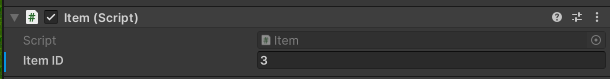
\includegraphics[scale=1]{Bilder/SerializeField.png}
\caption{Ein editierbares Feld in dem Unity Editor. Das Feld wird durch ein public Attribut, oder dem SerializeField Flag erzeugt.}
\label{fig:SerializeField}
\end{figure}
Eine Start Funktion ist in diesem Fall nicht notwendig. Die \texttt{Update} Methode bewegt das Item langsam an die übergebene Position. Time.deltaTime gibt die Zeit in Sekunden von dem letzten Bild bis zu dem momentanen Bild an. Dadurch wird die Bewegung linear.\\
Ein weiterer Teil der Spielesimulation ist die Bewegung der Items über das Förderband. Das Förderband übergibt die Position an das Item und bestimmt daher, in welche Richtung sich das Item bewegen soll:
\begin{lstlisting}[style=code, caption={Förderband Komponente OOP}]
public class BeltPath : MonoBehaviour
{
    private List<ConveyorComponent> beltPath = new ();
    //Referenzen auf die Komponenten des GameObjects werden geholt
    private InputConveyorComponent input 
        = GetComponent<InputConveyorComponent>();
    private OutputConveyorComponent output 
        = GetComponent<OutputConveyorComponent>();
    private float timeToMove = 2f;

    public void Update()
    {
        timeToMove -= Time.deltaTime;
        //Bewegung der Items wird alle 2 Sekunden durchgeführt
        if(timeToMove > 0) return;
        
        var lastBelt = beltPath[^1];
        if (!ReferenceEquals(lastBelt.item, null) && ReferenceEquals(output.GetItem(), null))
        {
            //Gegenstand von dem letzten Förderbandsegment auf den Output legen
            var item = lastBelt.item;
            var itemComponent = item.GetComponent<Item>();
            itemComponent.SetPosition(output.GetPosition());
            output.SetItem(item);
            lastBelt.item = null;
        }
        //Gegenstände von hinten nach vorne um ein Segment verschieben
        for (int i = beltPath.Count-2; i >= 0; i--)
        {
            var thisConveyor = beltPath[i];
            var lastConveyor = beltPath[i + 1];
            if (!ReferenceEquals(thisConveyor.item, null))
            {
                if (ReferenceEquals(lastConveyor.item, null))
                {
                    //Item kann verschoben werden
                    var item = thisConveyor.item;
                    var itemComponent = item.GetComponent<Item>();
                    lastConveyor.item = item;
                    //Position des Items aktualisieren
                    itemComponent.SetPosition(lastConveyor.pos);
                    thisConveyor.item = null;
                }
            }
        }
        var firstConveyor = beltPath[0];
        input.SetOccupied(!ReferenceEquals(firstConveyor.item, null));
        if (!ReferenceEquals(input.GetItem(), null) && ReferenceEquals(firstConveyor.item, null))
        {
            //Item wird von dem Input auf das erste Segment gelegt
            firstConveyor.item = input.GetItem();
            input.RemoveItem();
        }
        //Zeit wird wieder hochgestellt
        timeToMove += 2f;
    }
}
\end{lstlisting}
Für das Förderband wird eine Liste mit vorhandenen Segmenten, der Input, der Output und eine Zeit gespeichert. Die Zeit wird in der Start Methode initialisiert und der Input bzw. Output wird über die Funktion \glqq GetComponent()\grqq{} von dem GameObject geholt. In der \texttt{Update} Funktion wird zunächst nur die timeToMove Variable herunter gezählt. Sollte diese Variable unter Null fallen, werden alle Items von hinten nach vorne ein Segment weiter bewegt sofern dies möglich ist. Ist der Output nicht belegt wird ein vorhandenes Item in den Output gelegt. Items auf den einzelnen Segmenten werden nach weiterbewegt und wenn ein Item im Input liegt wird dies auf das erste Segment weiterbewegt. Immer wenn ein Item weitergegeben wird (egal ob an ein Segment, oder an den Output) wird auch die neue Position an das Item weitergegeben. Durch das bewegen der Items von hinten nach vorne verhindert man, dass sich Items nicht bewegen, obwohl sie es könnten.\\
Auf den Förderbändern sind Items richtige Objekte. In Gebäuden wird lediglich mit \texttt{ItemID's} gearbeitet, da man hier keine sichtbaren Objekte braucht. Um zu sehen, wie Items auf des Förderband gelangen und erstellt werden kann man sich die \texttt{Update} Methode einer Output Komponente eines Gebäudes anschauen:
\begin{lstlisting}[style=code, caption={Create Item OOP}]
void Update()
{
    //Wenn der Output leer ist gibt es nichts zu tun
    if(itemID == -1) return;
    outputGameObject ??= BuildingDictionary.Instance.GetGameObjectAtPosition(pos);
    if (ReferenceEquals(outputGameObject, null) ||
        !outputGameObject.TryGetComponent(out InputConveyorComponent input)) return;
    //Wenn Input des Förderbandes belegt ist wird auch keine
    //Änderung vorgenommen
    if(input.IsOccupied() || !ReferenceEquals(input.GetItem(), null)) return;
    var itemGameObject = Items.INSTANCE.GetItem(itemID);
    //Item wird erstellt
    var item = Instantiate(itemGameObject, new Vector3(pos.x, pos.y, -0.5f), Quaternion.identity);
    item.transform.localScale = new Vector3(0.5f, 0.5f, 0.5f);
    var itemComponent = item.GetComponent<Item>();
    itemComponent.SetPosition(pos);
    var inputConveyorComponent = outputGameObject.GetComponent<InputConveyorComponent>();
    //Input wird das Item zugewiesen
    inputConveyorComponent.SetItem(item);
    Item wird aus dem Output entfernt
    itemID = -1;
    itemCreated = true;
}
\end{lstlisting}
Da man sich im Objektorientierten, ohne weitere Vorkehrungen, immer auf dem \textit{Main Thread} befindet, lassen sich die Items direkt erstellen und dem Input übergeben. Das Zerstören von Items, also der Fall wenn Items von einem Förderband in ein Gebäude übergeben werden, funktioniert sehr ähnlich zu dem Erstellen von Items.